%% Ejemplo de la plantilla de latex para las diapositivas del Máster en IA 

%%%%%%%%%%%%%%%%%%%%%%%%%%%%
%% Valores para el ratio de aspecto: 43, 169 
%\documentclass[10pt, envcountsect, presentation, aspectratio=1610, hyperref={hypertexnames=true}]{beamer}
\documentclass[10pt, envcountsect, handout, aspectratio=1610, hyperref={hypertexnames=true}]{beamer}

%%%%%%%%%%%%%%%%%%%%%%%%%%%%

%%%%%%%%%%%%%%%%%%%%%%%%%%%%
%% Incluir fichero de estilo del máster
\input ../style/plantillaMasterIA.sty
%%%%%%%%%%%%%%%%%%%%%%%%%%%%

\addbibresource{../references.bib}



%\setbeameroption{show only notes} % Only notes
%\setbeameroption{show notes on second screen=right}  % Both
%\setbeamertemplate{note page}[compress]
\setbeameroption{hide notes} % Only slides




\renewcommand*\footnoterule{}
\setbeamerfont{footnote}{size=\tiny}




%\input{embed_video.tex}
%\usepackage{movie15}
\usepackage{multimedia}


%%%%%%%%%%%%%%%%%%%%%%%%%%%%
%% Información que aparecerá en la portada
\title[Aprendizaje por Refuerzo]{Aprendizaje por Refuerzo}
\subtitle{Bandido Multibrazo} % short title for footer

\author[L. D. Hernández] % Para el pie de página, poner los autores abreviados separados por comas.
{%
	\sc{Luis Daniel Hernández Molinero }\\ % Autor 1
	\textit{Ciencia de la Computación e Inteligencia Artificial}\\  % Area de conocimiento
	\textit{Dept. Ingeniería de la Información y las Comunicaciones}\\  % Departamento
	\\   % No dejes espacio entre esta línea y la llave siguiente 
}

\institute[DIIC]% % Poner las iniciales de los diferentes departamentos de los autores separadas por comas.
{
	\textit{Universidad de Murcia}
}

\newcounter{yearnext}
\setcounter{yearnext}{\the\year}
\addtocounter{yearnext}{-1}

\date{\arabic{yearnext}\ / \the\year\ } % Curso académico

%%%%%%%%%%%%%%%%%%%%%%%%%%%%%%%%%%
%% Contenido de las diapositivas
\setbeamerfont{normal text}{size=\normalsize} % Modifica el tamaño del texto de las diapositivas.
\AtBeginDocument{\usebeamerfont{normal text}}

%%%%%%%%%%%%%%%%%%%%%%%%%%%%%%%%%%

\begin{document}	

%%%%%%%%%%%%%%%%%%%%%%%%%%%%%%%%%%

%%%%%%%%%%%%%%%%%%%%%%%%%%%%%%%%%%

\begin{frame}[plain]
	\titlepage
\end{frame}

%%%%%%%%%%%%%%%%%%%%%%%%%%%%%%%%%%

\begin{frame}{Índice de Contenidos}
	\begin{multicols*}{2}
	\tableofcontents 
	\end{multicols*}
	
\end{frame}




%%%%%%%%%%%%%%%%%%%%%%%%%%%%%%%%%%%
%%%%%%%%%%%%%%%%%%%%%%%%%%%%%%%%%%%
%\begin{frame}{¿De qué va esto?}
%
%%\listofnotes
%
%
%\begin{abstract}
%\begin{itemize}
%\item Distinguir entre retroalimentación evaluativa de la instructiva.
%\item Planteaminto del problema del bandido multibrazo.
%\item Soluciones al problema del bandido multibrazo.
%	\begin{itemize}
%	\item Algoritmo Greedy
%	\item Algoritmos alternativos al Greedy
%	\end{itemize}
%\end{itemize}
%\end{abstract}
%
%
%\end{frame}






%%%%%%%%%%%%%%%%%%%%%%%%%%%%%%%%%%
%%%%%%%%%%%%%%%%%%%%%%%%%%%%%%%%%%

\begin{frame}{Introducción}{Retroalimentación Evaluativa vs Instructiva}
    \begin{block}{Retroalimentación Evaluativa}
        \begin{itemize}
            \item Se basa en la acción tomada, evaluando qué tan buena fue.
            \item No dice si la acción fue la mejor posible.
            \item Es típica en el aprendizaje por refuerzo
        \end{itemize}
    \end{block}

    \begin{block}{Retroalimentación Instructiva}
        \begin{itemize}
            \item Indica la acción correcta sin depender de la acción tomada.
            \item Es típica en el aprendizaje supervisado.
        \end{itemize}
    \end{block}

    \centering
    \textit{Estos dos tipos de retroalimentación son bastante distintos, pero pueden combinarse.}


% Cuarta transparencia: Enfoque del capítulo y entorno no asociativo

    \begin{itemize}
        %\item En este tema, se estudia el \textbf{aspecto evaluativo} del aprendizaje por refuerzo en un \textbf{entorno no asociativo}.
        %\item Un entorno no asociativo implica que no es necesario aprender a actuar en múltiples situaciones diferentes.
        \item El \textbf{problema del bandido multi-brazo} es una versión simplificada de un \textbf{entorno no asociativo}.
        
        Un agente debe elegir repetidamente entre diferentes opciones (o "brazos") sin conocer las recompensas.
        
        \item Este problema introduce \textbf{métodos básicos de aprendizaje} que se extenderán para el RL completo.
        
        %\item Hay que encontrar el equilibrio entre \textbf{exploración} (probar diferentes opciones) y \textbf{explotación} (elegir la mejor opción conocida).    
        \item Hay que encontrar el equilibrio entre \textbf{exploración} y \textbf{explotación}.    
        %\item Este enfoque nos permite ver con mayor claridad cómo difiere la retroalimentación evaluativa de la instructiva.
        \item El siguiente paso en el aprendizaje por refuerzo es considerar \textbf{entornos asociativos}.
    \end{itemize}



\end{frame}






%%%%%%%%%%%%%%%%%%%%%%%%%%%%%%%%%%
%%%%%%%%%%%%%%%%%%%%%%%%%%%%%%%%%%
\section{El Problema del Bandido Multibrazos}



%%%%%%%%%%%%%%%%%%%%%%%%%%%%%%%%%%
%%%%%%%%%%%%%%%%%%%%%%%%%%%%%%%%%%
\subsection{Planteamiento del problema}


%%%%%%%%%%%%%%%%%%%%%%%%%%%%%%%%%%
%%%%%%%%%%%%%%%%%%%%%%%%%%%%%%%%%%
\begin{frame}{Planteamiento del Problema}

\begin{columns}

\begin{column}{.7\textwidth}

\begin{block}{Planteamiento del Problema}
Para cada paso $t=1, 2,\ldots, T$
\begin{quote}
Tienes que elegir entre $k$ opciones diferentes (o acciones)\\
	\hfil Al elegir $a_t\in A$, recibes $r_t$
\end{quote}
\end{block}

\begin{block}{\faInfoCircle\/ ¿Por qué bandido $k$-brazos?}
\begin{itemize}
\item Un bandido es una máquina tragamonedas.
\item Un bandido de $k$-brazos es seleccionar la mejor entre $k$-máquinas.
\end{itemize}
\end{block}
\end{column}
\begin{column}{.3\textwidth}
\hfil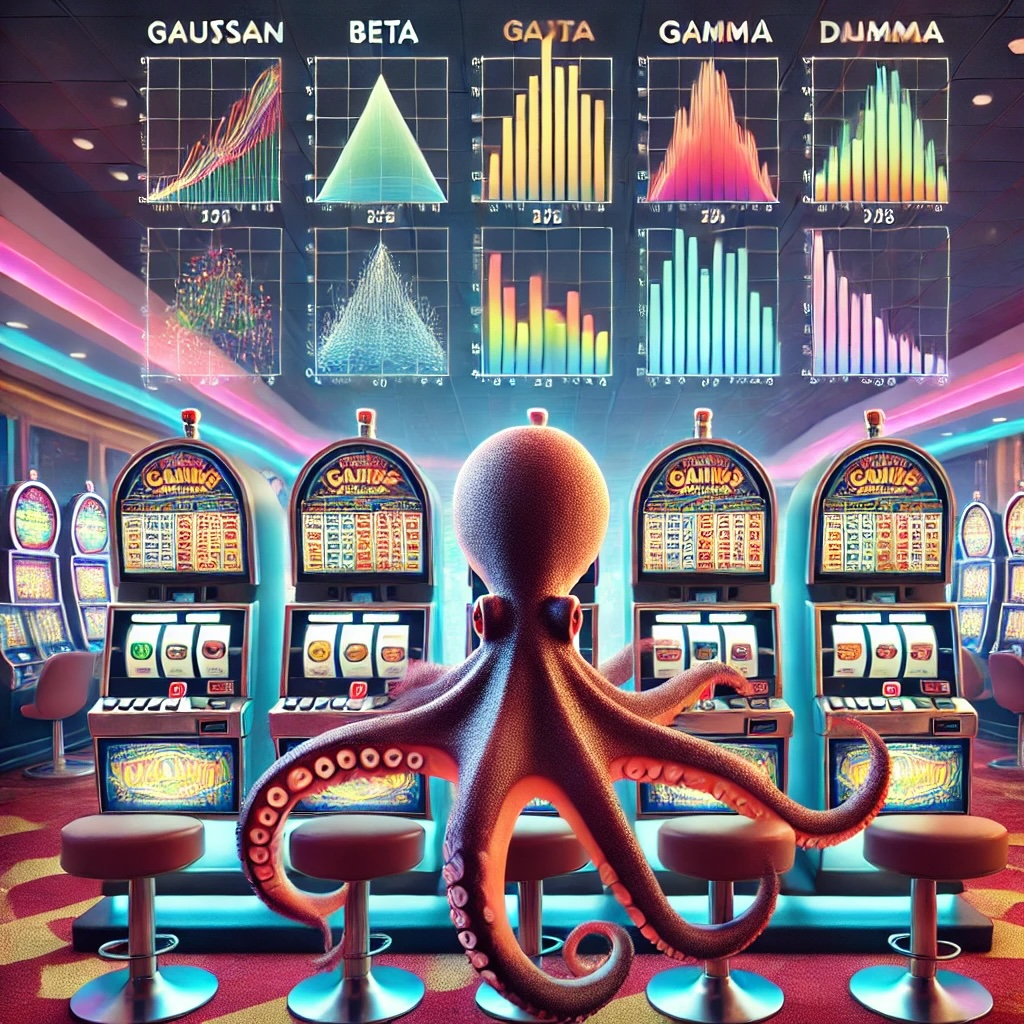
\includegraphics[width=\textwidth]{fig/pulpo}
\end{column}

\end{columns}



\begin{block}{Formalización. \citep{robbins1952} }
\begin{itemize}
\item 
Tenemos un conjunto $A$ de $K$ acciones (los brazos). $A=\{a_1,a_2,\ldots, a_k\}$


\item
Lo que sucede  en cada paso de tiempo, $t=1, 2, \ldots, T$ es que:

\begin{itemize}
\item 
	Elegiremos una acción $a_t\in A$

\item 
	Obtendremos una recompensa a partir de una distribución desconocida $r_t\sim Pr(r|a_t)$
\end{itemize}

\item
El objetivo, para cualquier algoritmo bandido, es maximizar la recompensa acumulada: $\sum_t r_t$
\end{itemize}

\end{block}

\end{frame}




%%%%%%%%%%%%%%%%%%%%%%%%%%%%%%%%%%
%%%%%%%%%%%%%%%%%%%%%%%%%%%%%%%%%%
\subsection{Ejemplos del problema del bandido multibrazos}


%%%%%%%%%%%%%%%%%%%%%%%%%%%%%%%%%%
%%%%%%%%%%%%%%%%%%%%%%%%%%%%%%%%%%
\begin{frame}{Ejemplos: A/B testing}

\begin{columns}
\begin{column}{.35\textwidth}

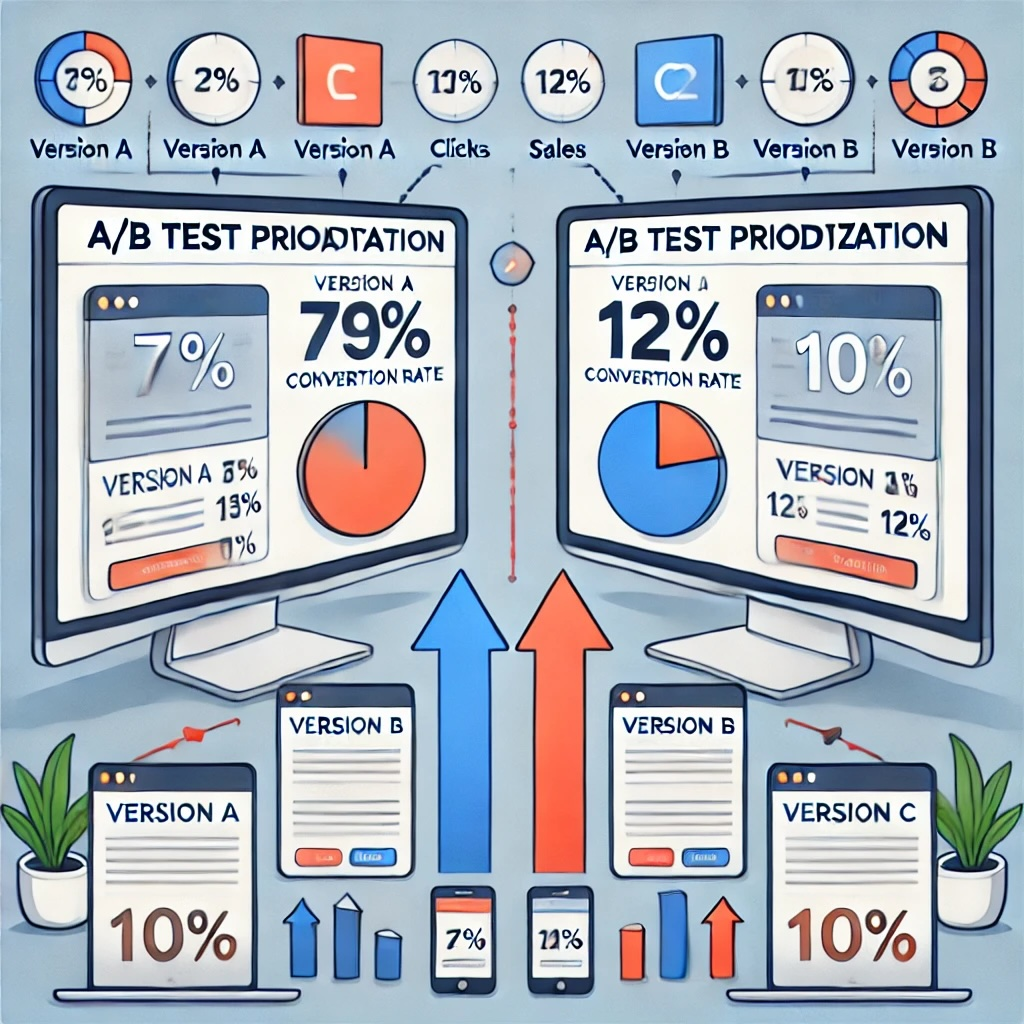
\includegraphics[width=\textwidth]{fig/testAB}

\end{column}


\begin{column}{.65\textwidth}

\begin{enumerate}
\item \textbf{Marketing Digital:} anuncios online, landing pages, e-mails, ...

\item \textbf{Diseño Web (Experiencia de Usuario):} interfaz de usuario (UI), flujos de usuarios, tiempos de carga, ...

\item \textbf{E-commerce:} checkout, productos recomendados, descuentos y promociones, ...

\item \textbf{Desarrollo de Producto:} características del producto, modelos de precios, interacciones, ...

\item \textbf{Redes Sociales:} contenidos, anuncios patrocinados, ...

\item \textbf{Publicidad Digital:} CTR (Click-through rate), conversión, ...

\item \textbf{Medios de Comunicación y Editoriales:} títulos de artículos, formatos de contenido, ...

\item \textbf{App. Móviles:} pantallas de bienvenida, interfaz en móviles, ... 

\item \textbf{Juegos en Línea:} monetización, características del juego, ...

\item \textbf{Medicina y Ciencias de la Salud:} ensayos clínicos, ...

\item etc
\end{enumerate}

\end{column}
\end{columns}

~

$T$-veces seleccionamos entre $K$-acciones y obtenemos una recompensa  $r_t\sim Pr(r|a_t)$. Objetivo: $\max \sum_t r_t$

\end{frame}






%%%%%%%%%%%%%%%%%%%%%%%%%%%%%%%%%%
%%%%%%%%%%%%%%%%%%%%%%%%%%%%%%%%%%
\begin{frame}{Ejemplos: Ensayos clínicos}

\begin{columns}
\begin{column}{.4\textwidth}

\centering
\textbf{Administración de Fármacos}

\hfil
\includegraphics[width=\textwidth]{fig/farmacos}

{\scriptsize $ $}

\end{column}


\begin{column}{.5\textwidth}

\hfil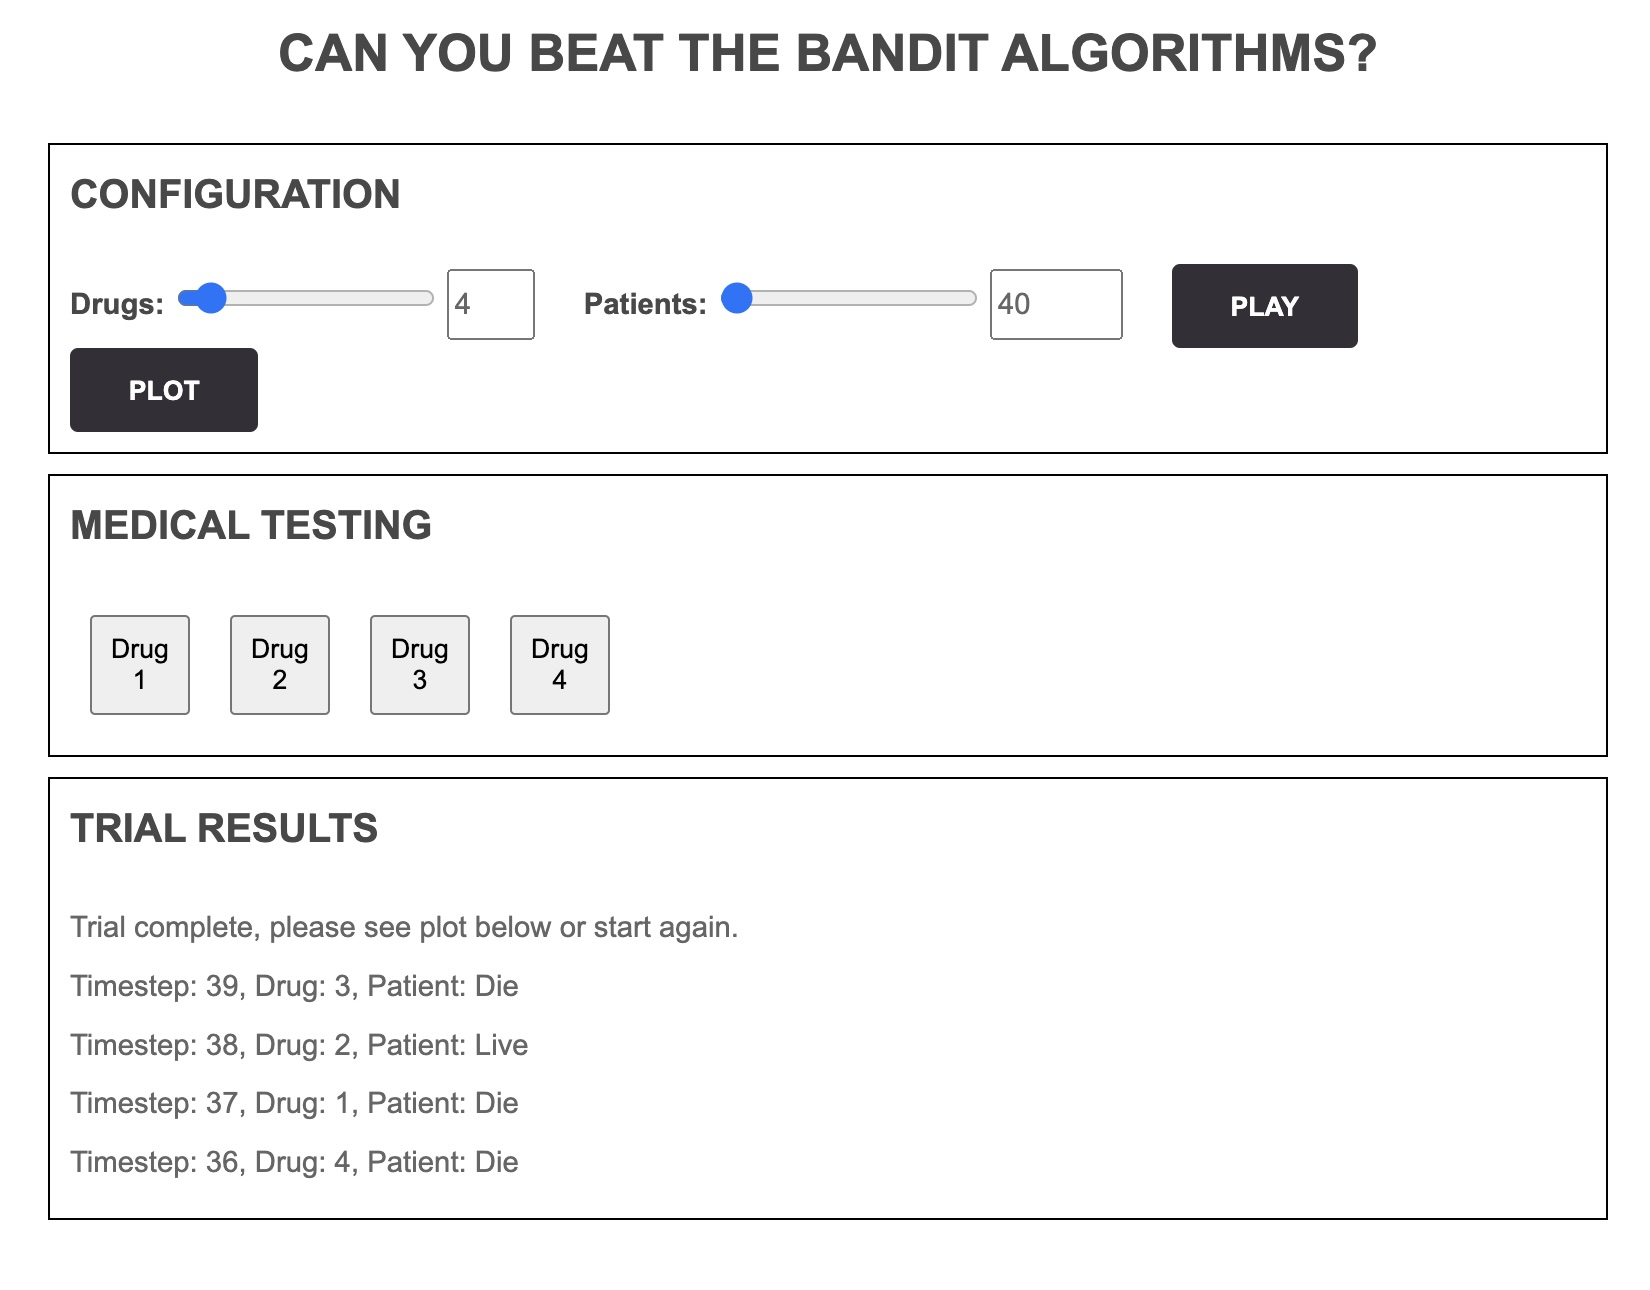
\includegraphics[width=\textwidth]{fig/juegoFarmacos}

\hfil {\scriptsize \url{https://iosband.github.io/2015/07/28/Beat-the-bandit.html}}



\end{column}
\end{columns}

~

~

$T$-veces seleccionamos entre $K$-acciones y obtenemos una recompensa  $r_t\sim Pr(r|a_t)$. Objetivo: $\max \sum_t r_t$

\end{frame}



%%%%%%%%%%%%%%%%%%%%%%%%%%%%%%%%%%
%%%%%%%%%%%%%%%%%%%%%%%%%%%%%%%%%%
\section{Soluciones al Problema del Bandido}

%%%%%%%%%%%%%%%%%%%%%%%%%%%%%%%%%%
%%%%%%%%%%%%%%%%%%%%%%%%%%%%%%%%%%
\subsection{Round-Robin}


\begin{frame}{Algoritmo Round-Robin}{Exploración}

\begin{itemize}
\item \textbf{Round-robin:} método que distribuye equitativamente o de forma cíclica recursos o tareas entre varios participantes, procesos o equipos.

\item Adaptación al problema del bandido multibrazo:
\begin{minipage}{.8\textwidth}
\begin{algoritmo}[H]	
\algsetup{linenosize=\tiny}		
\caption{\scriptsize{Algoritmo Round-Robin para el Problema del Bandido Multibrazo}}
\label{alg:Round-Robin}
	
\begin{algorithmic}[1]
\REQUIRE Número de acciones $T$, número de opciones (brazos) $K$
\STATE \textbf{Inicialización}: Recompensas acumuladas $R_k \gets 0$ para cada opción $k = 1, 2, \dots, K$
\STATE Inicializar el contador de elecciones $N_k \gets 0$ para cada opción $k = 1, 2, \dots, K$
\STATE Crear una cola circular de opciones $\{1, 2, \dots, K\}$
\FOR{$t = 1$ \textbf{hasta} $T$}
    \STATE Seleccionar la opción $k = ((t-1) \mod K) + 1$ (Round-Robin)
    \STATE Realizar la acción $k$ y observar la recompensa $r_k$
    \STATE Actualizar el valor de recompensa acumulada: $R_k \gets R_k + r_k$
    \STATE Actualizar el contador de elecciones: $N_k \gets N_k + 1$
\ENDFOR
\RETURN  Recompensas acumuladas $R_k$ y contadores $N_k$ para cada opción $k$
\end{algorithmic}

\end{algoritmo}
\end{minipage}

\item No es eficiente.
\end{itemize}

\end{frame}


%%%%%%%%%%%%%%%%%%%%%%%%%%%%%%%%%%
%%%%%%%%%%%%%%%%%%%%%%%%%%%%%%%%%%
\subsection{Métodos acción-valor}

%%%%%%%%%%%%%%%%%%%%%%%%%%%%%%%%%%
%%%%%%%%%%%%%%%%%%%%%%%%%%%%%%%%%%

\begin{frame}{Métodos Acción-Valor}{Método Promedio de Muestras}

\scalebox{1.2}{\begin{minipage}{0.8\textwidth}
\begin{itemize} 
\item \key{Valor de la acción $a$ :} 

 \fbox{\(q(a) \stackrel{\cdot}{=} \mathbb{E}[R_t | A_t = a]\)}\(=\sum_r r\cdot P(R_t=r|A_t=a)\).
	\begin{itemize} 
	\item $A_t$: la acción seleccionada en el paso de tiempo $t$,
	\item $R_t$: la recompensa correspondiente en el paso $t$,
	\item $\mathbb{E}$: el \textbf{operador de esperanza} o \textbf{valor esperado}.
	\end{itemize}

\

\item No conocemos las distribuciones de probabilidad: es necesario estimar $q(a)$.

\item \key{Métodos de Acción-Valor:} Los que usan estimaciones $Q_t(a)$ para tomar decisiones.

\item \key{Valor estimado de la acción $a$ según el método de promedio de muestras:}

\begin{align}
{Q}_t(a)  & = 
\frac{\sum_{i=1}^{t-1} R_i \cdot \mathbb{I}_{A_i = a}}{\sum_{i=1}^{t-1} \mathbb{I}_{A_i = a}}
\end{align}

\end{itemize}
\end{minipage}}


\TPMargin{0mm}%
\begin{textblock}{4.7}(10, 2.5)
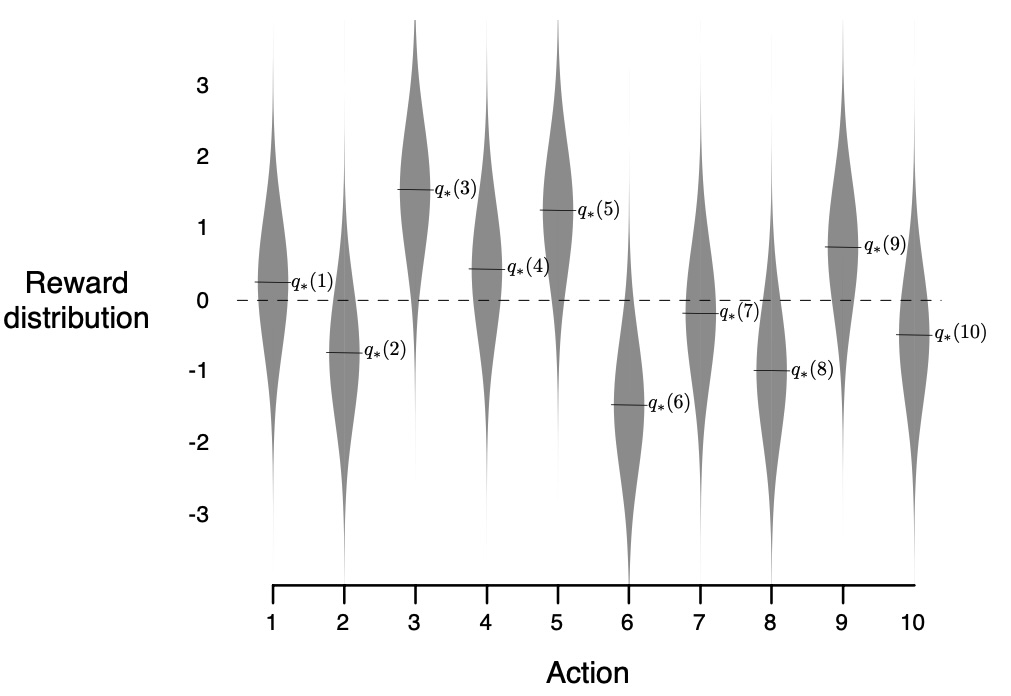
\includegraphics[width=1.2\textwidth, height=.35\textheight]{fig/bandit_example}
\end{textblock}


\end{frame}





%%%%%%%%%%%%%%%%%%%%%%%%%%%%%%%%%%
%%%%%%%%%%%%%%%%%%%%%%%%%%%%%%%%%%
\subsection{Algoritmo greedy}

%%%%%%%%%%%%%%%%%%%%%%%%%%%%%%%%%%
%%%%%%%%%%%%%%%%%%%%%%%%%%%%%%%%%%


%%%%%%%%%%%%%%%%%%%%%%%%%%%%%%%%%%
%%%%%%%%%%%%%%%%%%%%%%%%%%%%%%%%%%

\begin{frame}{Algoritmo greedy}{Explotación}

\begin{itemize}
\item \key{Algoritmo voraz:} Elegir aquella acción que tenga asociada una mayor recompensa.

\vskip -0.2cm
\begin{equation}
A_t \stackrel{\cdot}{=} \text{arg}_a \max Q_t(a)
\end{equation}

\vskip -0.8cm \hfil
\scalebox{0.9}{\begin{minipage}{.9\textwidth}
\begin{algoritmo}[H]	
\algsetup{linenosize=\tiny}		
\caption{\scriptsize{Algoritmo Greedy para el Problema del Bandido Multibrazo}}
\label{alg:Greedy}
	
\begin{algorithmic}[1]
\REQUIRE Número de acciones $T$, número de opciones (brazos) $K$
\STATE \textbf{Inicialización}: Recompensas acumuladas $R_k \gets 0$ y contador de elecciones $N_k \gets 0$ para cada opción $k = 1, 2, \dots, K$
\STATE Seleccionar cada opción $k$ \textbf{una vez} para inicializar la recompensa \textbf{(necesario)}
\FOR{$t = K+1$ \textbf{hasta} $T$}
    \STATE Seleccionar la opción $k$ que maximiza $\frac{R_k}{N_k}$ (la opción con mayor recompensa promedio)
    \STATE Realizar la acción $k$ y observar la recompensa $r_k$
    \STATE Actualizar el valor de recompensa acumulada: $R_k \gets R_k + r_k$
    \STATE Actualizar el contador de elecciones: $N_k \gets N_k + 1$
\ENDFOR
\RETURN Recompensas acumuladas $R_k$ y contadores $N_k$ para cada opción $k$
\end{algorithmic}

\end{algoritmo}
\end{minipage}}

\item\key{ Problema: } solo realiza explotaciones y no hace ningún intento de explorar.
\end{itemize}


\end{frame}




%%%%%%%%%%%%%%%%%%%%%%%%%%%%%%%%%%%%%%%%%%%%%%%%%%%%%%%%%%%%%%%%%%%%
%%%%%%%%%%%%%%%%%%%%%%%%%%%%%%%%%%%%%%%%%%%%%%%%%%%%%%%%%%%%%%%%%%%%

\subsection{Implementación incremental}

%%%%%%%%%%%%%%%%%%%%%%%%%%%%%%%%%%
%%%%%%%%%%%%%%%%%%%%%%%%%%%%%%%%%%

\begin{frame}{Implementación Incremental}

\begin{itemize}
\item Los métodos de acción-valor estiman los valores de la acciones como promedios de las recompensas.

\item ¿Se puede calcular el promedio de forma más eficiente el siguiente cálculo?
{\small
\begin{eqnarray}
 Q_{n+1}& = & \frac{1}{n}\sum_{i=1}^n R_i  \mbox{ (para 1 acción)}\nonumber \\
		& = & \frac{1}{n}\left( R_n + \sum_{i=1}^{n-1} R_i \right)  \nonumber \\
		& = & \frac{1}{n}\left( R_n + (n-1) \frac{1}{n-1} \sum_{i=1}^{n-1} R_i \right)  \nonumber \\
		& = & \frac{1}{n}\left( R_n + (n-1)  Q_n  \right)  \nonumber \\
		& = & \frac{1}{n}\left( R_n + n Q_n - Q_n  \right)  \nonumber \\
		& = & Q_n + \frac{1}{n} \left( R_n - Q_n \right) \label{eq:ActualizacionIncremental}
\end{eqnarray}
}

\item ${Nuevo Estimado} = {Viejo Estimado} + {Tama\text{\itñ}o del Paso} \cdot \left( {Objetivo} - {Viejo Estimado} \right).$
\end{itemize}


\end{frame}



%%%%%%%%%%%%%%%%%%%%%%%%%%%%%%%%%%
%%%%%%%%%%%%%%%%%%%%%%%%%%%%%%%%%%

\begin{frame}{Implementación incremental del algoritmo greedy}


\hfil
\scalebox{1}{
\begin{minipage}{.9\textwidth}
\begin{algorithm}[H]
\algsetup{linenosize=\tiny}		
\caption{\scriptsize{Algoritmo Greedy Incremental para el Problema del Bandido Multibrazo}}
\label{alg:GreedyIncremental}

\begin{algorithmic}[1]
\REQUIRE Número de acciones $T$, número de opciones (brazos) $K$
\STATE \textbf{Inicialización}: Promedio de recompensa estimado $Q_k \gets 0$ y contador de elecciones $N_k \gets 0$ para cada opción $k = 1, 2, \dots, K$
\STATE Seleccionar cada opción $k$ \textbf{una vez} para inicializar el promedio de recompensa \textbf{(necesario)}
\FOR{$t = K+1$ \textbf{hasta} $T$}
    \STATE Seleccionar la opción $k$ que maximiza $Q_k$ (la opción con mayor recompensa promedio estimada)
    \STATE Realizar la acción $k$ y observar la recompensa $r_k$
    \STATE Actualizar el promedio de recompensa estimado para la opción seleccionada:
    \[
    Q_k \gets Q_k + \frac{1}{N_k + 1} (r_k - Q_k)
    \]
    \STATE Actualizar el contador de elecciones: $N_k \gets N_k + 1$
\ENDFOR
\RETURN Promedios de recompensa $Q_k$ y contadores $N_k$ para cada opción $k$
\end{algorithmic}
\end{algorithm}
\end{minipage}}


\end{frame}










%%%%%%%%%%%%%%%%%%%%%%%%%%%%%%%%%%
%%%%%%%%%%%%%%%%%%%%%%%%%%%%%%%%%%
\subsection{Añadiendo Exploración}


%%%%%%%%%%%%%%%%%%%%%%%%%%%%%%%%%%%%%%%%%%%%%%%%%%%%%%%%%%%%%%%%%%%%
%%%%%%%%%%%%%%%%%%%%%%%%%%%%%%%%%%%%%%%%%%%%%%%%%%%%%%%%%%%%%%%%%%%%

\subsubsection{$\epsilon$-greedy}

%%%%%%%%%%%%%%%%%%%%%%%%%%%%%%%%%%
%%%%%%%%%%%%%%%%%%%%%%%%%%%%%%%%%%

\begin{frame}{Algoritmo $\epsilon$-greedy}

\begin{itemize}
\item Ser codicioso (explotar), pero no siempre (explorar) con una probabilidad $\epsilon$.

\vskip -0.4cm
\hfil
\scalebox{.8}{
\begin{minipage}{1.2\textwidth}
\begin{algorithm}[H]	
\caption{Algoritmo $\epsilon$-Greedy para el Problema del Bandido Multibrazo}
\label{alg:epsilon-Greedy}
	
\begin{algorithmic}[1]
\REQUIRE Número de acciones $T$, número de opciones (brazos) $K$, parámetro de exploración $\epsilon$
\STATE \textbf{Inicialización}: Recompensas acumuladas $R_k \gets 0$ y contador de elecciones $N_k \gets 0$ para cada opción $k = 1, 2, \dots, K$
\STATE Seleccionar cada opción $k$ una vez para inicializar la recompensa \textbf{(opcional)}
\FOR{$t = K+1$ \textbf{hasta} $T$}
    \STATE Generar un número aleatorio $p$ entre $0$ y $1$
    \IF{$p < \epsilon$} 
        \STATE \textbf{Exploración:} Seleccionar una opción $k$ aleatoria entre $1$ y $K$
    \ELSE
        \STATE \textbf{Explotación:} Seleccionar la opción $k$ que maximiza $\frac{R_k}{N_k}$ (la opción con mayor recompensa promedio)
    \ENDIF
    \STATE Realizar la acción $k$ y observar la recompensa $r_k$
    \STATE Actualizar el valor de recompensa acumulada: $R_k \gets R_k + r_k$
    \STATE Actualizar el contador de elecciones: $N_k \gets N_k + 1$
\ENDFOR
\RETURN Recompensas acumuladas $R_k$ y contadores $N_k$ para cada opción $k$
\end{algorithmic}

\end{algorithm}
\end{minipage}}

\item $\lim_{t\rightarrow \infty} Q_t(a) = q(a)$

\item \textit{\color{red}Ejercicio.} Para el caso de dos acciones y \( \epsilon = 0.5 \), ¿cuál es la probabilidad de que se seleccione la acción codiciosa?

\end{itemize}



\end{frame}





%%%%%%%%%%%%%%%%%%%%%%%%%%%%%%%%%%
%%%%%%%%%%%%%%%%%%%%%%%%%%%%%%%%%%

\begin{frame}{Implementación incremental de $\epsilon$-greedy}


\begin{algorithm}[H]	
\caption{Algoritmo $\epsilon$-Greedy Incremental para el Problema del Bandido Multibrazo}
\label{alg:epsilon-Greedy-Incremental}
	
\begin{algorithmic}[1]
\STATE \textbf{Inicialización:}
\FOR{$a = 1$ \TO $k$}
    \STATE $Q(a) \gets 0$
    \STATE $N(a) \gets 0$
\ENDFOR

\WHILE{True}
    \STATE Seleccionar una acción $A$:
    \STATE $A \gets
    \begin{cases}
        \arg\max_a Q(a) & \text{con probabilidad } 1 - \epsilon \mbox{\hspace{3cm}\color{black}  (rompiendo aleatoriamente)} \\
        \text{una acción aleatoria} & \text{con probabilidad } \epsilon 
    \end{cases}$
    
    \STATE $R \gets \text{bandido}(A)$ \hfill (Obtener la recompensa de la acción seleccionada)
    \STATE $N(A) \gets N(A) + 1$ \hfill (Actualizar el contador de la acción)
    \STATE $Q(A) \gets Q(A) + \ds \frac{1}{N(A)} \cdot (R - Q(A))$ \hfill (Actualizar el valor estimado)
\ENDWHILE

\end{algorithmic}
\end{algorithm}

\end{frame}



%%%%%%%%%%%%%%%%%%%%%%%%%%%%%%%%%%
%%%%%%%%%%%%%%%%%%%%%%%%%%%%%%%%%%

\begin{frame}{Comparativa $\epsilon$-greedy}

\begin{columns}
\begin{column}{.58\textwidth}
\hfil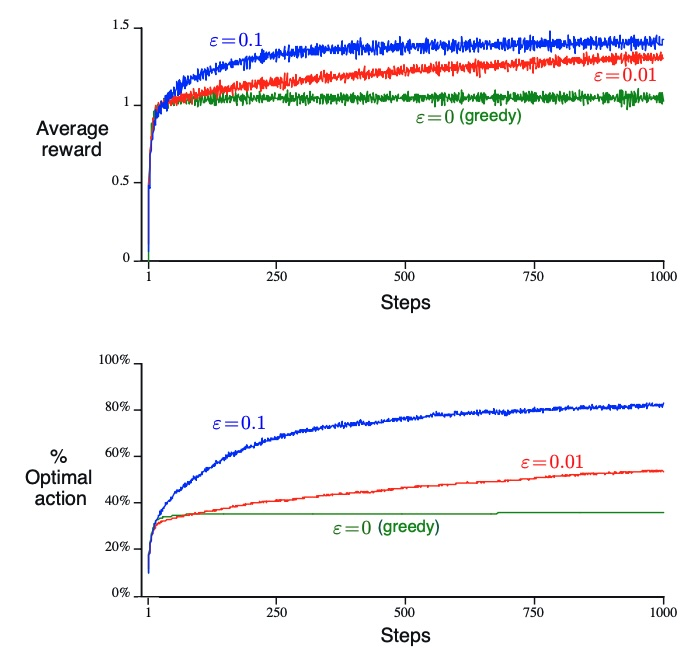
\includegraphics[width=\textwidth]{fig/epsilon_greedy_comparison}
\end{column}
\begin{column}{.42\textwidth}
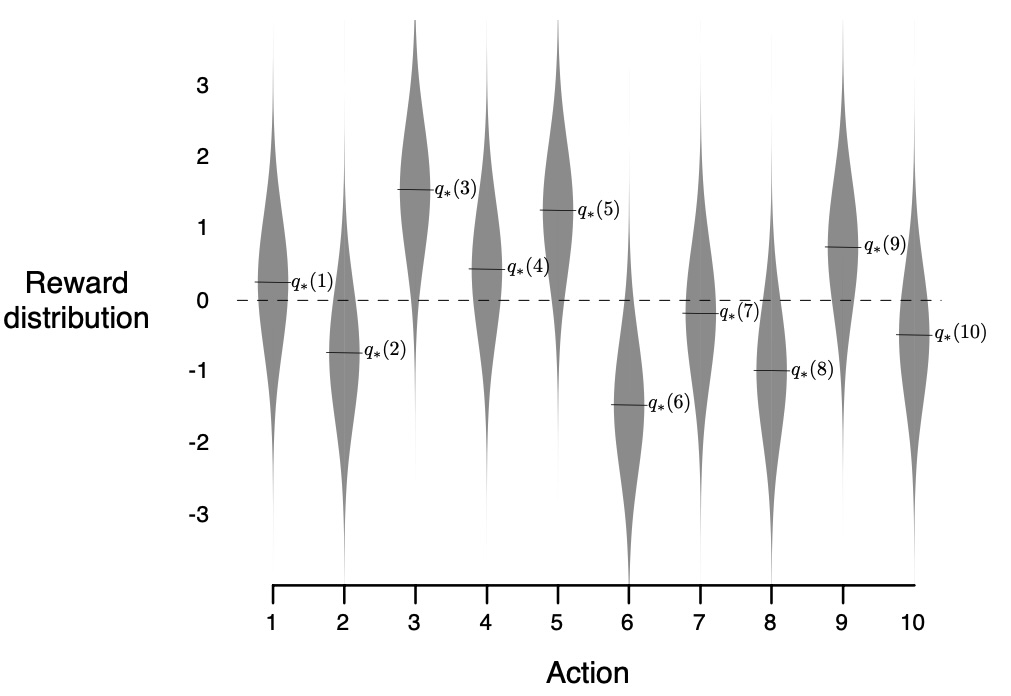
\includegraphics[width=\textwidth]{fig/bandit_example}

~

~

\hfil Figuras de \cite{Sutton2018}
\end{column}
\end{columns}

\end{frame}




\subsubsection{Métodos optimistas}

%%%%%%%%%%%%%%%%%%%%%%%%%%%%%%%%%%
%%%%%%%%%%%%%%%%%%%%%%%%%%%%%%%%%%

\begin{frame}{Método de Valores Iniciales Optimistas}

\scalebox{1.4}{
\begin{minipage}{.7\textwidth}
\begin{itemize}
\item Constan de dos pasos generales:
	\begin{enumerate}
	\item Inicializar las estiamaciones $Q_1(a)$ a un valor extremadamente optimista.
	\item Aplicar un algoritmo voraz.
	\end{enumerate}
	
\item Se espera que haya una gran exploración al principio y después se centre en la explotación.

\item Algoritmo Voraz Optimista. Ejemplos:
	\begin{itemize}
	\item Fármacos: $Q_1(a)=1$
	\item 10-brazos: $Q_1(a)=5$
	\end{itemize}
	
\end{itemize}
\end{minipage}}


\end{frame}



%%%%%%%%%%%%%%%%%%%%%%%%%%%%%%%%%%%%%%%%%%%%%%%%%%%%%%%%%%%%%%%%%%%%
%%%%%%%%%%%%%%%%%%%%%%%%%%%%%%%%%%%%%%%%%%%%%%%%%%%%%%%%%%%%%%%%%%%%

\subsubsection{$\epsilon$-decaimiento}



%%%%%%%%%%%%%%%%%%%%%%%%%%%%%%%%%%
%%%%%%%%%%%%%%%%%%%%%%%%%%%%%%%%%%

\begin{frame}{Algoritmo $\epsilon$-decaimiento}

\begin{itemize}
\item A medida que el agente acumula experiencia, el objetivo es hacer una mayor explotación de las mejores acciones conocidas y reducir la exploración con probabilidad $\epsilon$. 

\vskip -0.4cm
\hfil
\scalebox{.9}{
\begin{minipage}{.9\textwidth}
\begin{algorithm}[H]
\caption{$\epsilon$-decaimiento para selección de acciones}\label{alg:epsilon_decay}

\begin{algorithmic}[1]

\REQUIRE Nº de acciones $K$, Nº de pasos $T$, valor inicial de exploración $\epsilon_0$, tasa de decaimiento $\lambda$, valor mínimo de exploración $\epsilon_{\text{min}}$.

\STATE \textbf{Inicialización}: Recompensas acumuladas $R_k \gets 0$ y contador de elecciones $N_k \gets 0$ para cada acción $k = 1, 2, \dots, K$

\STATE Generar cada opción $k$ una vez para inicializar la recompensa.

\FOR{$t = 1$ \textbf{hasta} $T$}
    \STATE Calcular $\epsilon_t = \max(\epsilon_{\text{min}}, f(t, \epsilon_0, \lambda))$.
    
    \STATE \textbf{Con probabilidad} $\epsilon_t$:
    \STATE \hspace{1em} Seleccionar una acción $k$ al azar de entre las $K$ acciones (exploración)
    
    \STATE \textbf{Con probabilidad} $1 - \epsilon_t$:
    \STATE \hspace{1em} Seleccionar la acción $k = \arg\max \frac{R_k}{N_k}$ (explotación)
    
    \STATE Realizar la acción $k$ y observar la recompensa $r_k$
    \STATE Actualizar la recompensa acumulada: $R_k \gets R_k + r_k$
    \STATE Actualizar el contador de elecciones: $N_k \gets N_k + 1$
\ENDFOR

\STATE \textbf{Salida}: Recompensas acumuladas $R_k$ y contadores $N_k$ para cada acción $k$

\end{algorithmic}
\end{algorithm}
\end{minipage}}
\end{itemize}



\end{frame}







%%%%%%%%%%%%%%%%%%%%%%%%%%%%%%%%%%
%%%%%%%%%%%%%%%%%%%%%%%%%%%%%%%%%%

\begin{frame}[fragile]{Algoritmo $\epsilon$-decaimiento}{Funciones de decaimiento}

\begin{columns}

\begin{column}{.4\textwidth}


\begin{itemize}
	
\item Decaimiento Lineal:
   \[
   f(t, \epsilon_0, \lambda) = \epsilon_0 - t \cdot \lambda
   \]

\item Decaimiento Exponencial:
   \[
   f(t, \epsilon_0, \lambda) = \epsilon_0 \cdot e^{-\lambda t}
   \]

\item Decaimiento Inversamente Proporcional:
   \[
   f(t, \epsilon_0, \lambda) = \frac{\epsilon_0}{1 + \lambda t}
   \]
\end{itemize}

\end{column}

\begin{column}{.6\textwidth}
\begin{pycode}
import numpy as np
import matplotlib.pyplot as plt

# Parámetros
epsilon_0 = 1.0
lambda_ = 0.01
t_values = np.linspace(0, 200, 200)

# Funciones de decaimiento
def linear_decay(t, epsilon_0, lambda_):
    return np.maximum(epsilon_0 - t * lambda_, 0)

def exponential_decay(t, epsilon_0, lambda_):
    return epsilon_0 * np.exp(-lambda_ * t)

def inverse_decay(t, epsilon_0, lambda_):
    return epsilon_0 / (1 + lambda_ * t)

# Cálculo de los valores
epsilon_linear = linear_decay(t_values, epsilon_0, lambda_)
epsilon_exponential = exponential_decay(t_values, epsilon_0, lambda_)
epsilon_inverse = inverse_decay(t_values, epsilon_0, lambda_)

# Gráfico
plt.figure(figsize=(8, 5))
plt.plot(t_values, epsilon_linear, label="Decaimiento Lineal")
plt.plot(t_values, epsilon_exponential, label="Decaimiento Exponencial")
plt.plot(t_values, epsilon_inverse, label="Decaimiento Inversamente Proporcional")
plt.xlabel("Paso $t$")
plt.ylabel("$\epsilon_t$")
plt.title("Comparación de Funciones de Decaimiento de $\epsilon$")
plt.legend()
plt.grid(True)

# Guardar el gráfico
plt.savefig("fig/epsilon_decay_comparison.png")
\end{pycode}

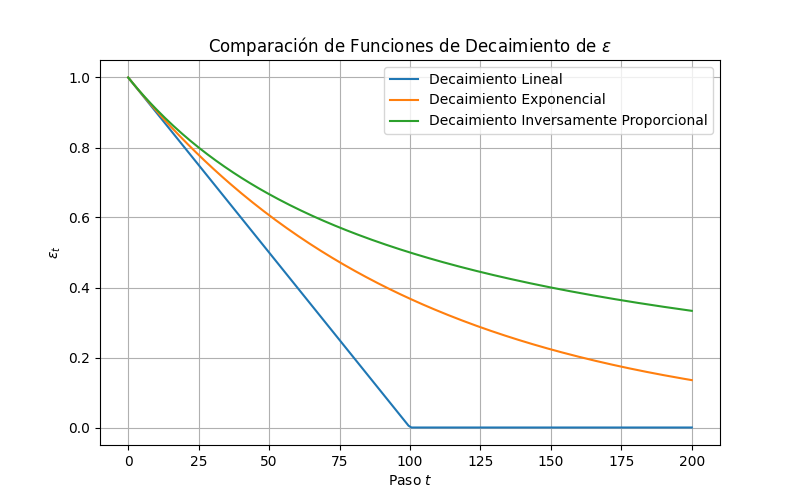
\includegraphics[width=\textwidth]{fig/epsilon_decay_comparison.png}

\hfill\begin{minipage}{.4\textwidth} \footnotesize
$\bullet$ $\epsilon_0 = 1.0$ \quad 
$\bullet$ $\lambda = 0.01$

%\begin{itemize}
%\item[$\bullet$] $\epsilon_0 = 1.0$
%\item[$\bullet$] $\lambda = 0.01$
%\end{itemize}
\end{minipage}

\end{column}

\end{columns}

~

~


\hfil Con probabilidad $\epsilon_t = \max(\epsilon_{\text{min}}, f(t, \epsilon_0, \lambda))$ tomamos una acción al azar.



\end{frame}


%%%%%%%%%%%%%%%%%%%%%%%%%%%%%%%%%%%%%%%%%%%%%%%%%%%%%%%%%%%%%%%%%%%%
%%%%%%%%%%%%%%%%%%%%%%%%%%%%%%%%%%%%%%%%%%%%%%%%%%%%%%%%%%%%%%%%%%%%

\subsection{Métodos índice}

%%%%%%%%%%%%%%%%%%%%%%%%%%%%%%%%%%%%%%%%%%%%%%%%%%%%%%%%%%%%%%%%%%%%
%%%%%%%%%%%%%%%%%%%%%%%%%%%%%%%%%%%%%%%%%%%%%%%%%%%%%%%%%%%%%%%%%%%%

\subsubsection{Midiendo la eficiencia}

%%%%%%%%%%%%%%%%%%%%%%%%%%%%%%%%%%
%%%%%%%%%%%%%%%%%%%%%%%%%%%%%%%%%%

\begin{frame}{¿Cómo medir la eficiencia de un algoritmo?}

\begin{itemize}
\item Para comparar algoritmos entre sí ¿es mejor el que haya obtenido más recompensa?

\item Arrepentimiento: $R_T=\sum_{t=1}^T (q^*-r_t)=q^* T - \sum_{t=1}^T r_t$ con $q^*=\max_{a\in A} q(a)$

\hfil
\scalebox{1}{
\begin{minipage}{.8\textwidth}
\begin{algorithm}[H]
\caption{Cálculo de arrepentimiento}\label{alg:arrepentimiento}

\begin{algorithmic}[1]

%\REQUIRE $num\_arms \leftarrow 10$ \COMMENT{Número de brazos}
%\REQUIRE $num\_steps \leftarrow 1000$ \COMMENT{Número de pasos}
%\REQUIRE $true\_means \leftarrow$ \texttt{np.random.rand}$(num\_arms)$ \COMMENT{Recompensas verdaderas para cada brazo}

\REQUIRE Nº de pasos $T$, Nº de brazos $arms$, $reward\gets 0$, \\ ~ \qquad recompensas verdaderas $q(a)=rand(0,max)$

\FOR{$t = 1$ \textbf{hasta} $T$}
	\STATE $arm \gets bandit(t)$
	\STATE $r \gets random.normal(q(arm), 1.0)$  \COMMENT{Supuesto que es $N(\mu, 1)$}
    \STATE $reward \gets reward + r$
\ENDFOR

\STATE $QMAX = \max_{a\in arms}{q(a)}$

\STATE $regret \gets QMAX * T - reward $
\ENSURE $regret$

\end{algorithmic}
\end{algorithm}
\end{minipage}}


\item Pero la expresión a estudiar es:  \hfil \key{Arrepentimiento (esperado)}

\hfil $\ds \mathbb{E}[R_T]=\ds \mathbb{E}\big [ \sum_{i=1}^T (q^*-r_t) \big]=q^* T - \sum_{t=1}^T \mathbb{E}(r_t)$

\end{itemize}

\end{frame}


%%%%%%%%%%%%%%%%%%%%%%%%%%%%%%%%%%
%%%%%%%%%%%%%%%%%%%%%%%%%%%%%%%%%%

\begin{frame}{Arrepentimiento (Esperado)}

\begin{itemize}
\item Un desarrollo conveniente \citep{bonald2017bandits}: 

$
\begin{array}{rll}
{\color{red} L_T}=\mathbb{E}[R_T] & = \ds \mathbb{E}\big [ {\color{red}\sum_{i=1}^T} (q^*-r_t) \big] &\ds = T \, \mathbb{E}[r|a^*] - \sum_{t=1}^T \mathbb{E}[r|a_t] \\ 
% & &
%				\qquad \textcolor{black}{
%				q^*=\max_{a\in A} q(a)  \text{ y } q(a) \stackrel{\cdot}{=} \mathbb{E}[R | A = a]
%				} \\
	&\ds = T q^* - \sum_{t=1}^T \mathbb{E}[q(a_t)] 
	 &\ds = T q^* - \sum_{t=1}^T {\color{red} \sum_{a\in A}}\mathbb{E}[q(a) \cdot \mathbb{I}_{a_t=a}] \\
	&\ds = T q^* -  \sum_{a\in A} q(a) \sum_{t=1}^T \mathbb{E}[ \mathbb{I}_{a_t=a}] 
	 &\ds = T q^* -  \sum_{a\in A} q(a) \mathbb{E}\big[ \sum_{t=1}^T \mathbb{I}_{a_t=a} \big] \\
	&\ds = T q^* -  \sum_{a\in A} q(a) \mathbb{E}\big[ N_T(a) \big]
%	&\ds = \sum_{a\in A}  q^* \; \mathbb{E}\big[ N_T(a) \big] -  \sum_{a\in A}   q(a)) \; \mathbb{E}\big[ N_T(a) \big] \\
	&\ds = {\color{red} \sum_{a\in A}}  (q^* -  q(a)) \; \mathbb{E}\big[ N_T(a) \big] 
\end{array}
$

\item $\ds \mathbb{E}\big[ N_T(a) \big]=\sum_{t=1}^T \mathbb{E}[ \mathbb{I}_{a_t=a}]=\sum_{i=1}^T \big[ 1\cdot P(a_t=a) + 0\cdot P(a_t\not=a) \big]= \sum_{t=1}^T P(a_t=a) = \sum_{t=1}^T P(a) = T \cdot P(a) $


\end{itemize}	

\end{frame}



%%%%%%%%%%%%%%%%%%%%%%%%%%%%%%%%%%
%%%%%%%%%%%%%%%%%%%%%%%%%%%%%%%%%%

\begin{frame}{Arrepentimiento}

\begin{itemize}
\item \cite{Lai1985} demuestra que bajo ciertas condiciones se cumple

\hfil$
\ds \liminf_{T\rightarrow \infty }\frac{\sum_{i: \mu_i < \mu^*} (\mu^* - \mu_i) E[n_i]}{\ln(T)} \geq \sum_{i: \mu_i < \mu^*} \frac{\mu^* - \mu_i}{I(\mu_i, \mu^*)} = Cte
$

\begin{itemize}
\item El numerador es $L_T$: $q^*=\mu^*$, $q(a_i)=\mu_i$, $E[n_i]=\mathbb{E}[N_T(a_i)]$.

\item Nota: Si \( a_n = (-1)^n + \frac{1}{n} \), entonces \( \ds \lim_{n \to \infty} a_n \) no existe, pero \( \ds \liminf_{n \to \infty} a_n = -1 \).

\item Consecuencia: {\large $\ds L_T \geq Cte \cdot \ln(T)$}

\end{itemize}

~

\item \key[red]{Requisito}: \hfil {\large $ \mathbb{E}[n_i] \geq
    \frac{ \ln(T) }{I(\mu_i, \mu^*)}  $  }

\begin{itemize}
\item Divergencia  de Kullback-Leibler: $\ds I(\mu_j, \mu^*) = \ds \int_{-\infty}^{+\infty} \log\left(\frac{p_i(x)}{p^*(x)}\right) p_j(x)\ dx$ 

	\begin{itemize}
	\item Divergencia  de Kullback-Leibler de $j$ respecto de la óptima.
	\item No es conmutativa.
	\end{itemize}
	
\item Se espera que el número de veces que el brazo $i$ haya sido elegido $ \mathbb{E}[n_i] $ sea superior a cierto valor.

\end{itemize}

\end{itemize}	


\end{frame}




%%%%%%%%%%%%%%%%%%%%%%%%%%%%%%%%%%%%%%%%%%%%%%%%%%%%%%%%%%%%%%%%%%%%
%%%%%%%%%%%%%%%%%%%%%%%%%%%%%%%%%%%%%%%%%%%%%%%%%%%%%%%%%%%%%%%%%%%%

\subsubsection{Métodos UCB (Upper Confidence Bound)}

%%%%%%%%%%%%%%%%%%%%%%%%%%%%%%%%%%
%%%%%%%%%%%%%%%%%%%%%%%%%%%%%%%%%%

\begin{frame}{Métodos UCB (Upper Confidence Bound)}{Políticas de índice}

\scalebox{1.15}{
\begin{minipage}{.86\textwidth}
\begin{itemize}


\item $\epsilon$-greddy puede explorar seleccionando una acción mala. Entonces, podríamos usar \key{algún tipo de medida} que indique un equilibrio entre el valor conocido y la incertidumbre.

\item \cite{Agrawal1995} introdujo una clase genérica de \key{políticas de índice} denominadas límites superiores de confianza (upper confidence bounds, UCB), basado en \cite{Lai1985}.

\item El método de \key{límites de confianza superiores} (UCB) mide el potencial de cada brazo con un índice para cada política (brazo/acción) que está formado por la suma de dos términos.

\hfil $ ucb(a)=Q(a) + u(a) $

\begin{itemize}
\item \key{Término de explotación}, $Q(a)$
\item \key{Término de exploración}, $u(a)$ (límite superior)
	\begin{itemize}
    \item Una medida de la incertidumbre asociada con la estimación de la recompensa promedio del brazo $a$.
	\item Debe ser más pequeño conforme aumente el número de veces que se selecciona la acción $a$.
	\end{itemize} 
\item Si $q(a)\in[Q(a)-u(a),\ Q(a)+u(a)]$, entonces $q(a)\leq  Q(a)+u(a)$   
\end{itemize}

\item \key{Siempre selecciona la acción más codiciosa} para maximizar el límite superior de confianza 

\hfil $\ds a_t = arg\ \max_{a\in A} ucb(a)$
\end{itemize}
\end{minipage}}

\end{frame}



%%%%%%%%%%%%%%%%%%%%%%%%%%%%%%%%%%
%%%%%%%%%%%%%%%%%%%%%%%%%%%%%%%%%%

\begin{frame}{Método UCB1}

%\scalebox{1.15}{
%\begin{minipage}{.86\textwidth}
\begin{itemize}
\item Existen \key{varias versiones} del algoritmo Upper Confidence Bound (UCB). 

\item \cite{Auer2002}: \key{UCB1}
	\begin{itemize}
	\item Es la primera versión concreta y práctica del concepto de UCB 
	\item La designación "1"\/ por ser la primera y distinguirla de otras variantes.
	\end{itemize}

\item \key{Desigualdad de Hoeffding:} $Pr\left (|\bar {X} - \mu| \ge \varepsilon \right)  \le 2 e^{-2 n \varepsilon^2}$
	\begin{itemize}
	\item $\bar {X}$ es la media de los valores $\mapsto Q_t(a)$ estimación del valor de la acción \( a \) en el tiempo \( t \).
	\item $\mu$ es la media de la distribución $\mapsto q(a)$ valor de la acción.
	\item $\varepsilon$ es el valor máximo para el que queremos medir la probabilidad $\mapsto u(a)$ limite superior de confianza
	\item $n$ es el número de muestras $\mapsto N_t(a)$ número de veces que la acción $a$ ha sido seleccionada antes de $t$.
	\end{itemize}

\item \key{Definiendo}  $\varepsilon = \sqrt {\frac {1} {2n} \ln {\frac {2} {\alpha}}}$, obtenemos
$
Pr\left (|\bar {X} - \mu| \ge \varepsilon \right) \le 
2 e^{-2 n \left( \sqrt {\frac {1} {2n} \ln {\frac {2} {\alpha}}} \right) ^2} = 
e^{-\ln \frac{2}{\alpha}}=\frac{2}{\alpha}
$

\item \key{UCB1 establece} $\ds\frac{2}{\alpha}=t^{-4}$, con $t$ el número total de acciones.

\begin{columns}
\begin{column}{.03\textwidth}
\end{column}

\begin{column}{.45\textwidth}
\begin{align*}
u(a) & = \varepsilon =  \sqrt {\frac {1} {2N_t(a)} \ln {\frac {2} {\alpha}}} = \sqrt {\frac {1} {2N_t(a)} \ln {t^4}} = \sqrt {\frac {2 \ln{t} } {N_t(a)} } \\
A_t  & = arg\ \max_{a\in A} Q_t(a) + \sqrt {\frac {2 \ln{t} } {N_t(a)}}
\end{align*}
\end{column}

\begin{column}{.35\textwidth}
$ \text{Valor UCB1}(a) = Q(a) + c \times \sqrt{\frac{\ln t}{N(a)}} $
\begin{itemize}
        \item \( c \): parámetro de ajuste que controla el grado de exploración (usualmente se toma \( c = 1 \)).
\end{itemize}

~

\end{column}
\end{columns}
\end{itemize}
\end{frame}





%%%%%%%%%%%%%%%%%%%%%%%%%%%%%%%%%%
%%%%%%%%%%%%%%%%%%%%%%%%%%%%%%%%%%

\begin{frame}{Método UCB2}

%\scalebox{1.15}{
%\begin{minipage}{.86\textwidth}
\begin{itemize}
\item En el mismo artículo, \cite{Auer2002} propone UCB2
\item $\text{Valor UCB2}(a) = Q(a) +$ \Large $\sqrt{\frac{(1 + \alpha) \ln \left(\frac{e\cdot t}{\tau(k_a)}\right)}{2 \tau(k_a)}}$
    \begin{itemize}
        \item \( 0<\alpha<1 \): parámetro de ajuste para el balance entre exploración y explotación.
		\item \( k_a \): número de épocas de la  acción \( a \).
        \item \( \tau(k_a) = \left\lceil (1 + \alpha)^{k_a} \right\rceil  \): determina el número de veces que la acción \( a \) será seleccionada en un época.
    \end{itemize}


\hfil
\begin{minipage}{.8\textwidth}
\begin{algorithm}[H]	
\caption{Algoritmo UCB2}
\label{alg:UCB2}
	
\begin{algorithmic}[1]  \small
    \STATE \textbf{Inicialización de valores:} $0<\alpha<1$, $t \gets 0$, $N(a) \gets 0$, $Q(a) \gets 0$, $k_a \gets 0$
    \STATE \textbf{Inicialización de recompensas:} Selecciona cada acción una vez, actualizando $t$, $N(a) \gets 1$, $Q(a)$
    \WHILE{el criterio de parada no se cumpla ($t<T$)}
        \STATE \textbf{Seleccionar la Acción con el Índice Máximo:} \( a \gets \arg \max_{a'} \text{UCB2}(a') \)
        \STATE \textbf{Ejecuta la acción} $a$ \textbf{el número de veces que indique su bloque} de tiempo \\ \hfil \( \left\lceil \tau(k_a + 1) - \tau(k_a) \right\rceil \) \\ Actualizando $t \gets t + 1$, $N(a) \gets N(a) + 1$ y el promedio de recompensas \( Q(a) \).
        \STATE Actualizar $k_a \gets k_a + 1$
    \ENDWHILE
\end{algorithmic}
\end{algorithm}
\end{minipage}


\end{itemize}

\end{frame}






%%%%%%%%%%%%%%%%%%%%%%%%%%%%%%%%%%
%%%%%%%%%%%%%%%%%%%%%%%%%%%%%%%%%%

\begin{frame}{Variantes UCB1-Tuned}

%\scalebox{1.15}{
%\begin{minipage}{.86\textwidth}
\begin{itemize}
\item \textbf{UCB1-Tuned} $\text{Valor UCB1-Tuned}(a) = Q(a) + \sqrt{\frac{\ln t}{N(a)} \cdot \min \left( \frac{1}{4}, V(a) + \sqrt{\frac{2 \ln t}{N(a)}} \right)}$
    \begin{itemize}
     \item \( V(a) \): estimación de la varianza empírica de las recompensas para la acción \( a \).
        
        \begin{itemize}
        \item La varianza empírica de las recompensas se calcula como: $ V(a) = \frac{1}{N(a)} \sum_{i=1}^{N(a)} (r_i - Q(a))^2$
        \item Alternativamente, $ V(a) = \frac{1}{N(a)} \sum_{i=1}^{N(a)} r_i^2 - \left(Q(a)\right)^2$
		\item Esta última fórmula puede ser computacionalmente más estable y conveniente en algunos casos.
		\end{itemize}

		
		
	\item Expresión incremental:
	\begin{columns}
	\begin{column}{0\textwidth}
	\end{column}
	\begin{column}{.42\textwidth}
		\begin{enumerate}
		\item[\textbf{1.}]  Actualización del Promedio Incremental dado el promedio anterior \( Q_N \) y la nueva recompensa \( r_{N+1} \):
		\[
		Q_{N+1} = Q_N + \frac{r_{N+1} - Q_N}{N+1}
		\]

		\item[\textbf{2.}] Actualización de la Varianza Incremental. 
		\[
		V_{N+1} = V_N + \frac{(r_{N+1} - Q_N)(r_{N+1} - Q_{N+1})}{N+1}
		\]
		\end{enumerate}
	\end{column}
	\begin{column}{.52\textwidth}
		\noindent {\footnotesize \textbf{2'.} Actualización de la Varianza Incremental.}
		\begin{enumerate}
		\item Mantener dos sumas acumuladas: \\
			$-$ Suma de las recompensas: \( S_N = \sum_{i=1}^{N} r_i \) \\
			$-$ Suma de los cuadrados de las recompensas: \( S_N^{(2)} = \sum_{i=1}^{N} r_i^2 \)
			
		\item Actualizar las sumas: \\
			$-$ \(S_{N+1} = S_N + r_{N+1}\) \\
			$-$  \( S_{N+1}^{(2)} = S_N^{(2)} + r_{N+1}^2\)

		\item Actualizar la varianza \( V_{N+1} \):
   			\[
   			V_{N+1} = \frac{S_{N+1}^{(2)}}{N+1} - \left( \frac{S_{N+1}}{N+1} \right)^2
  			 \]
		\end{enumerate}
	\end{column}
	\end{columns}	
    \end{itemize}
\end{itemize}

\end{frame}


%%%%%%%%%%%%%%%%%%%%%%%%%%%%%%%%%%
%%%%%%%%%%%%%%%%%%%%%%%%%%%%%%%%%%

\begin{frame}{Más variantes UCB}
\begin{itemize}


\item \textbf{UCB-Improved o UCB-V (UCB-Variance)} $\text{Valor UCB-Improved}(a) = Q(a) + \sqrt{\frac{\sigma(a)^2 \ln t}{N(a)}}$
    \begin{itemize}
        \item \( \sigma(a)^2 \): varianza estimada de las recompensas para la acción \( a \).
    \end{itemize}
    
\item \textbf{UCB with Decaying Exploration} $\text{Valor UCB-Decay}(a) = Q(a) + \frac{c \ln t}{N(a)^{\alpha}}$
    \begin{itemize}
        \item \( \alpha \): parámetro que controla la tasa de decaimiento de la exploración (usualmente \( 0 < \alpha < 1 \)).
    \end{itemize}
    
\item \textbf{UCB-Confidence Bound Adjustment (UCB-C)} $\text{Valor UCB-C}(a) = Q(a) + \sqrt{\frac{\ln(t + 1) + f(N(a))}{N(a)}}$
    \begin{itemize}
        \item \( f(N(a)) \): función ajustable para cambiar el peso del término de exploración en función de \( N(a) \), que puede depender del problema.
    \end{itemize}
\end{itemize}

\end{frame}



%%%%%%%%%%%%%%%%%%%%%%%%%%%%%%%%%%%%%%%%%%%%%%%%%%%%%%%%%%%%%%%%%%%%
%%%%%%%%%%%%%%%%%%%%%%%%%%%%%%%%%%%%%%%%%%%%%%%%%%%%%%%%%%%%%%%%%%%%

\subsection{Métodos de Ascenso del Gradiente}



%%%%%%%%%%%%%%%%%%%%%%%%%%%%%%%%%%
%%%%%%%%%%%%%%%%%%%%%%%%%%%%%%%%%%

\begin{frame}{Método Softmax}

\begin{itemize}
\item $\epsilon$-Greedy selecciona bandidos aleatoriamente, experimentando con todos con la misma probabilidad.
    \begin{itemize}
    \item Ignora que algunas esperanzas medias crezcan más que  otras.
    \end{itemize}

\item Idea: \key{Asignar una probabilidad} a cada acción proporcional al valor de la recompensa esperada actual.

\hfil \textbf{Función de Gibbs} (softmax): $\ds P(A_t=a)= \frac{e^{Q_t(a) / \tau}}{\sum_{b=1}^{k} e^{Q_t(b)/ \tau}} \stackrel{\cdot}{=} \pi_t(a)$
\hfill
\(
\text{Pr}(x_i) = \frac{e^{-\frac{E(x_i)}{kT}}}{\sum_{j} e^{-\frac{E(x_j)}{kT}}}
\)


\end{itemize}

%\begin{algorithm}

%\end{algorithm}


\begin{minipage}{.8\textwidth}
\begin{algoritmo}[H]	
\algsetup{linenosize=\tiny}		
\caption{\scriptsize{Algoritmo Softmax para el Problema del Bandido Multibrazo}}
\label{alg:Softmax} \footnotesize

\begin{algorithmic}[1]
    \STATE \textbf{Inicialización:}
    \STATE Para cada acción $a$, establecer la recompensa promedio inicial $Q_0(a) = 0$
    \STATE Establecer una valor $\tau > 0$
    \FOR{cada tiempo $t = 1, 2, 3, \ldots$}
    	\FOR{cada tiempo $k = 1, 2, \ldots, K$ (número de brazos)}
        	\STATE Calcular las probabilidades de selección para cada acción $a$:
        	\( \ds
        	\pi_t(a) = \frac{e^{Q_t(a)/\tau}}{\sum_{b=1}^k e^{Q_t(b)/\tau}}
        	\)
		\ENDFOR
        \STATE Seleccionar una acción $A_t$ de acuerdo con la distribución de probabilidad $\pi_t(a)$
        \STATE Recibir la recompensa $R_t$ correspondiente a la acción $A_t$
        \STATE Actualizar la recompensa promedio:
        \( \ds
        {Q}_t(a) = {Q}_{t-1}(a) + \frac{1}{k} (R_t - {Q}_{t-1}(a))
        \)
    \ENDFOR
\end{algorithmic}

\end{algoritmo}
\end{minipage}

\end{frame}



%%%%%%%%%%%%%%%%%%%%%%%%%%%%%%%%%%
%%%%%%%%%%%%%%%%%%%%%%%%%%%%%%%%%%

\begin{frame}{Método de Gradiente de Preferencias}

\begin{itemize}
\item En \cite{Sutton2018}  se propone utilizar
\( \ds
\pi_t(a) \stackrel{\cdot}{=} \frac{e^{H_t(a)}}{\sum_{b=1}^{K} e^{H_t(b)}}
\)
\begin{itemize}
\item \( H_t(a) \in \mathbb{R} \) es una preferencia numérica para cada acción \( a \)
\item A mayor preferencia (no recompensa), más frecuente se tomará la acción.
\end{itemize}

\item Objetivo: aprender $H_t(a)$ mediante Método del Ascenso de Gradiente Estocástico.
$$\theta_{t+1} = \theta_t(x_t) + \alpha \nabla f(\theta_t, x_t) \quad 
\Longrightarrow  \quad
H_{t+1}(a) = H_t(a) + \alpha \frac{\partial E[R_t]}{\partial H_t(a)} \text{ con  }  E[R_t] = \ds \sum_{x} \pi_t(x) q(x) 
$$

\item Actualizar las preferencias para cada acción tras  seleccionar la acción \( A_t \) y recibir la recompensa \( R_t \):

\begin{align*}
H_{t+1}(A_t) & \stackrel{\cdot}{=} H_t(A_t) + \alpha (R_t - \bar{R}_t)(1 - \pi_t(A_t)), \text{ y}  \\
H_{t+1}(a) & \stackrel{\cdot}{=} H_t(a) - \alpha (R_t - \bar{R}_t)\pi_t(a), \quad \text{para todo } a \neq A_t
\end{align*}



\end{itemize}

\end{frame}




%%%%%%%%%%%%%%%%%%%%%%%%%%%%%%%%%%%%%%%%%%%%%%%%%%%%%%%%%%%%%%%%%%%%
%%%%%%%%%%%%%%%%%%%%%%%%%%%%%%%%%%%%%%%%%%%%%%%%%%%%%%%%%%%%%%%%%%%%

\subsection{Métodos Bayesianos}


%%%%%%%%%%%%%%%%%%%%%%%%%%%%%%%%%%%%%%%%%%%%%%%%%%%%%%%%%%%%%%%%%%%%
%%%%%%%%%%%%%%%%%%%%%%%%%%%%%%%%%%%%%%%%%%%%%%%%%%%%%%%%%%%%%%%%%%%%

\subsubsection{Muestreo de Thomson}

%%%%%%%%%%%%%%%%%%%%%%%%%%%%%%%%%%
%%%%%%%%%%%%%%%%%%%%%%%%%%%%%%%%%%

\begin{frame}{Muestreo de Thomson}
\begin{itemize}
\item Es un método alternativo a los métodos optimistas frente a la incertidumbre.

\item \cite{thompson1933likelihood} propone

\begin{quote}
... although serious objection can otherwise be raised to argument
based upon a small number of observations. Indeed, the fact that such objection
can never be eliminated entirely—no matter how great the number of observations—
suggested the possible value of seeking other modes of operation than that of taking
a large number of observations before analysis or any attempt to direct our course.
\end{quote}


\begin{itemize}
\item Y es que la estadística bayesiana estaba muy mal vista 
\item Recomendado: \citet{Armero2022}.
\end{itemize}

\item \key{Planteamiento bayesiano.}

    \begin{enumerate}
        \item Modelar cada opción \(a \in A\) con una distribución de probabilidad \(P(\theta_a)\), donde:
        \begin{itemize}
            \item \(\theta_a\) representa el parámetro de éxito de la opción.
        \end{itemize}
        \item En cada iteración:
        \begin{itemize}
            \item Seleccionar la mejor opción de acuerdo a su distribución de probabilidad
            \item Considerar el nuevo dato observado $D_a$
            \item Aplicar T. Bayes $\ds P(\theta_{a} | D_a) = \frac{P(D_a | \theta_{a}) P(\theta_{a})}{P(D_a)}$
        \end{itemize}
    \end{enumerate}


\end{itemize}
\end{frame}


%%%%%%%%%%%%%%%%%%%%%%%%%%%%%%%%%%
%%%%%%%%%%%%%%%%%%%%%%%%%%%%%%%%%%

\begin{frame}{\textit{Bandit} de Bernoulli con Perspectiva Bayesiana}


\begin{itemize}
	\item $k\in{1, \ldots, K}$. Tenemos $K$-acciones.
	\item $r_k \sim \text{Bernoulli}(\theta_k)$

	\begin{itemize}
		\item $\theta=(\theta_1,\ldots, \theta_K)$ es desconocida pero fija en el tiempo (no cambia).
	    \item \(r_k \in \{0, 1\}\) es la recompensa obtenida al seleccionar la acción \(k\),
    	\item \(\theta_k \in [0, 1]\) es la probabilidad de éxito asociada a la acción \(k\),
    	\item \(\text{Bernoulli}(\theta_k)\) denota la distribución Bernoulli con parámetro \(\theta_k\).
	
		\hfil \(P(r_k = 1 | \theta_k) = \theta_k, \quad P(r_k = 0 | \theta_k) = 1 - \theta_k. \)

    \end{itemize}
    
    \item \begin{enumerate}
    \item $\forall k \quad r_k \sim \mathbb{P}(\theta_k)$  
    \item $x_1 \mapsto r_1 \in \{0, 1\} \mapsto P(r_1 | x_1, \theta) = \theta_1$
	\item $x_2 \mapsto r_2 \in \{0, 1\} \mapsto P(r_2 | x_1, \theta_1) = \theta_2$
    \item etc ...
    \end{enumerate}
    
    \item \key{Inicialmente}, el parámetro $\theta_k$ será uniforme (al azar). $\theta_k \sim U(0, 1)=Beta(\alpha_k=1,\beta_k=1)$
    
    \hfil\( p(\theta_k) = \ds \frac{\Gamma(\alpha_k + \beta_k)}{\Gamma(\alpha_k)\Gamma(\beta_k)} \theta_k^{\alpha_k - 1}(1 - \theta_k)^{\beta_k - 1}\qquad  \Gamma(x) = \int_{0}^{\infty} t^{x-1} e^{-t} \, dt.\)
    
    %\item Conforme se recopilan observaciones, l
    \item La distribución se actualiza según la \key{Regla de Bayes}: $f(\theta|x) \propto L(x|\theta) f(\theta)$
    
     \hfil \textbf{\small Si $\theta\sim Beta(\alpha, \beta)$, $L(x|\theta)\sim Bernouilli(\theta)$, entonces $\theta|x \sim Beta(\alpha + x, \beta + 1-x)$}
    
    
    \item \key{Regla de actualización:}
    
    \hfil\(
(\alpha_k, \beta_k) \leftarrow
\begin{cases} 
(\alpha_k, \beta_k) & \text{si } x_t \neq k, \\
(\alpha_k, \beta_k) + (r_t, 1 - r_t) & \text{si } x_t = k.
\end{cases}
\)

\end{itemize}
\end{frame}


%%%%%%%%%%%%%%%%%%%%%%%%%%%%%%%%%%
%%%%%%%%%%%%%%%%%%%%%%%%%%%%%%%%%%


\begin{frame}{Algoritmos Bayesianos para el \textit{Bandit} de Bernoulli}{\cite{Russo2018TS}}

\scalebox{0.7}{
\begin{minipage}{1.4\textwidth}
\begin{columns} 
\begin{column}{.5\textwidth}
\begin{algorithm}[H]
\caption{Greedy para Beta-Bernoulli}
\begin{algorithmic}[1]
\REQUIRE $K$, $\alpha$, $\beta$
\FOR{$t = 1, 2, \dots$}
    \STATE \COMMENT{Estimar modelo:}
    \FOR{$k = 1, \dots, K$}
        \STATE $\hat{\theta}_k \leftarrow \frac{\alpha_k}{\alpha_k + \beta_k}$
    \ENDFOR
    \STATE
    \STATE \COMMENT{Seleccionar y aplicar acción:}
    \STATE $x_t \leftarrow \arg\max_k \hat{\theta}_k$
    \STATE Aplicar $x_t$ y observar $r_t$
    \STATE
    \STATE \COMMENT{Actualizar distribución:}
    \STATE $(\alpha_{x_t}, \beta_{x_t}) \leftarrow (\alpha_{x_t} + r_t, \beta_{x_t} + 1 - r_t)$
\ENDFOR
\end{algorithmic}
\end{algorithm}
\end{column}

\begin{column}{.5\textwidth}
\begin{algorithm}[H]
\caption{Muestreo de Thompson para Beta-Bernoulli}
\begin{algorithmic}[1]
\REQUIRE $K$, $\alpha$, $\beta$
\FOR{$t = 1, 2, \dots$}
    \STATE \COMMENT{Muestrear modelo:}
    \FOR{$k = 1, \dots, K$}
        \STATE Muestrear $\hat{\theta}_k \sim \text{Beta}(\alpha_k, \beta_k)$
    \ENDFOR
    \STATE
    \STATE \COMMENT{Seleccionar y aplicar acción:}
    \STATE $x_t \leftarrow \arg\max_k \hat{\theta}_k$
    \STATE Aplicar $x_t$ y observar $r_t$
    \STATE
    \STATE \COMMENT{Actualizar distribución:}
    \STATE $(\alpha_{x_t}, \beta_{x_t}) \leftarrow (\alpha_{x_t} + r_t, \beta_{x_t} + 1 - r_t)$
\ENDFOR
\end{algorithmic}
\end{algorithm}
\end{column}
\end{columns}
\end{minipage}}


\hfil\begin{columns} 
\begin{column}{.2\textwidth}
\textbf{Ejemplo:}
\begin{itemize} \small
\item[] $\theta_1 = 0,9$
\item[] $\theta_2 = 0,8$ 
\item[] $\theta_3 = 0,7$
\item[] $10000$ simulaciones
\item[] $T=1000$
\end{itemize}
\end{column}

\begin{column}{.6\textwidth}
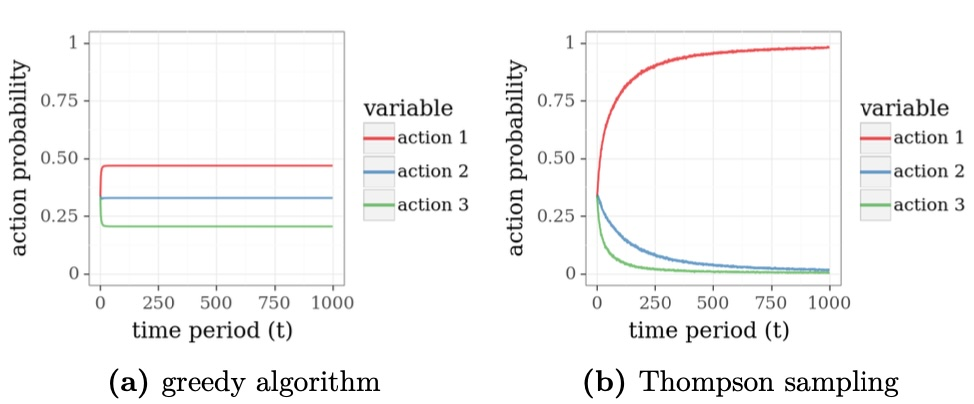
\includegraphics[height=.35\textheight]{fig/Bern-TS}
\end{column}
\end{columns}

\end{frame}




%%%%%%%%%%%%%%%%%%%%%%%%%%%%%%%%%%
%%%%%%%%%%%%%%%%%%%%%%%%%%%%%%%%%%


\begin{frame}{Muestreo de Thompson General}

\begin{itemize}
\item \key{Componentes} del problema general:
	\begin{itemize}
	\item Acciones: $x_1, x_2, x_3, \dots \in X$
	\item Tras una acción $x_t$, se observa un resultado $y_t \sim q_\theta(\cdot | x_t)$.
	\item $\theta$ es incierta, pero tiene su propia distribución $\theta \sim p$
	\item Se obtiene una recompensa $r_t=r(y_t)$, con $r$ función conocida.
	\end{itemize}
	
	En Beta-Bernoulli: $r(y)=y$, $y_t=r_t \sim q_\theta=Bern(\theta)$  y $\theta \sim p=Beta(1, 1)$
	
\item \key{Recompensa esperada} para $\hat{\theta}$: 
\(
\mathbb{E}_{q_{\hat{\theta}}}[r(y_t) | x_t = x] = \sum_o q_{\hat{\theta}}(o | x) r(o).
\)

\item \key{Teorema de Bayes:} $\ds p \gets 
P_{p,q}(\theta = u | x_t, y_t) = \frac{p(u) q_u(y_t | x_t)}{\sum_v p(v) q_v(y_t | x_t)}.
$

\end{itemize}

\scalebox{0.9}{
\begin{minipage}{1.1\textwidth}
\begin{columns} 
\begin{column}{.5\textwidth}
\begin{algorithm}[H]
\caption{\textit{Greedy}($X, p, q, r$)}
\begin{algorithmic}[1]
\FOR{$t = 1, 2, \dots$}
    \STATE \textbf{Estimar modelo:} $\hat{\theta} \leftarrow \mathbb{E}_p[\theta]$
    \STATE \textbf{Seleccionar y aplicar acción:}
    \STATE $x_t \leftarrow \arg\max_{x \in X} \mathbb{E}_{q_{\hat{\theta}}}[r(y_t) | x_t = x]$
    \STATE Aplicar $x_t$ y observar $y_t$
    \STATE \textbf{Actualizar distribución:} $p \leftarrow P_{p,q}(\theta \in \cdot | x_t, y_t)$
\ENDFOR
\end{algorithmic}
\end{algorithm}

\end{column}

\begin{column}{.5\textwidth}
\begin{algorithm}[H]
\caption{Thompson($X, p, q, r$)}
\begin{algorithmic}[1]
\FOR{$t = 1, 2, \dots$}
    \STATE \textbf{Muestrear modelo:} Muestrear $\hat{\theta} \sim p$
    \STATE \textbf{Seleccionar y aplicar acción:}
    \STATE $x_t \leftarrow \arg\max_{x \in X} \mathbb{E}_{q_{\hat{\theta}}}[r(y_t) | x_t = x]$
    \STATE Aplicar $x_t$ y observar $y_t$
    \STATE \textbf{Actualizar distribución:} $p \leftarrow P_{p,q}(\theta \in \cdot | x_t, y_t)$
\ENDFOR
\end{algorithmic}
\end{algorithm}
\end{column}
\end{columns}
\end{minipage}}

\end{frame}



%%%%%%%%%%%%%%%%%%%%%%%%%%%%%%%%%%%%%%%%%%%%%%%%%%%%%%%%%%%%%%%%%%%%
%%%%%%%%%%%%%%%%%%%%%%%%%%%%%%%%%%%%%%%%%%%%%%%%%%%%%%%%%%%%%%%%%%%%

\subsubsection{UCB Bayesiano}


\begin{frame}{UCB Bayesiano}
\begin{itemize}
\item Recuerda:
	\begin{itemize}
	\item $ucb(a)=Q(a) + u(a) $
	\item Término de explotación, $Q(a)$ (el promedio de las recompensas)
	\item Término de exploración, $u(a)$ (límite superior)
	\item $\ds a_t = arg\ \max_{a\in A} ucb(a)$
	\end{itemize}

\item \key{Si conocemos la distribución}, usar $ucb(a) = \mu(a) + \gamma \sigma(a) $
	\begin{itemize}
	\item $\mu(a)$ es la media de recompensas obtenidas por $a$.
	\item $\sigma(a)$ es la desviación estándar de la distribución.
	\item $\gamma$ determina el número de desviaciones.
	\end{itemize}
	
\item \textbf{Ejemplo.} Si $a\sim Beta(\alpha, \beta)$, se sabe que
$\mu(a) =\frac{\alpha}{\alpha + \beta}$  y que $\sigma(a) =\sqrt{\frac{\alpha \cdot \beta}{(\alpha + \beta)^2 \cdot (\alpha + \beta + 1)}}$

Con lo que el índice de cada decisión vendrá dada por:

\hfil $
ucbbayes(a) = \frac{\alpha_j}{\alpha_j + \beta_j} + \gamma \; \cdot \; \sqrt{\frac{\alpha_j \cdot \beta_j}{(\alpha_j + \beta_j)^2 \cdot (\alpha_j + \beta_j + 1)}}
$
\end{itemize}

\end{frame}



%%%%%%%%%%%%%%%%%%%%%%%%%%%%%%%%%%%%%%%%%%%%%%%%%%%%%%%%%%%%%%%%%%%%
%%%%%%%%%%%%%%%%%%%%%%%%%%%%%%%%%%%%%%%%%%%%%%%%%%%%%%%%%%%%%%%%%%%%

\section{Conclusiones}

%%%%%%%%%%%%%%%%%%%%%%%%%%%%%%%%%%
%%%%%%%%%%%%%%%%%%%%%%%%%%%%%%%%%%

\begin{frame}{Conclusiones}
	
\scalebox{1.1}{\begin{minipage}{.8\textwidth}
	\begin{itemize}
	\item 	\textbf{\large Conclusiones principales:}
	\begin{itemize}
		\item El problema del bandido multibrazos es clave para entender la toma de decisiones bajo incertidumbre.
		\item Algoritmos como el greedy son simples pero efectivos en contextos limitados.
		\item Métodos avanzados ofrecen mejores resultados, especialmente cuando la exploración es crítica.
		\item La elección del algoritmo depende del equilibrio entre precisión, eficiencia y contexto específico.
	\end{itemize}
%	\textbf{Consecuencias más amplias:}
%	\begin{itemize}
%		\item Promueve el desarrollo de sistemas autónomos más inteligentes y adaptativos.
%		\item Estimula la investigación en modelos híbridos que combinen técnicas de aprendizaje supervisado y por refuerzo.
%		\item Impacta directamente en campos como la medicina personalizada, donde decisiones críticas deben tomarse con datos limitados.
%		\item Influye en el diseño de políticas públicas basadas en datos dinámicos, optimizando recursos y resultados.
%		\item Contribuye a la eficiencia en la industria, como en la gestión de inventarios y optimización logística.
%	\end{itemize}
	\item \textbf{\large Aplicaciones:}
	\begin{itemize}
		\item Publicidad en línea (A/B testing).
		\item Optimización de sistemas en tiempo real.
		\item Sistemas de recomendación y más.
	\end{itemize}
\end{itemize}
\end{minipage}}
	
	\nocite{analyticslane2021bandit}
	\nocite{silver2015lecture9}

\end{frame}






%%%%%%%%%%%%%%%%%%%%%%%%%%%%%%%%%%
%%%%%%%%%%%%%%%%%%%%%%%%%%%%%%%%%%
% BIBLIOGRAFÍA
%%%%%%%%%%%%%%%%%%%%%%%%%%%%%%%%%%
%%%%%%%%%%%%%%%%%%%%%%%%%%%%%%%%%%


%%%%%%%%%%%%%%%%%%%%%%%%%%%%%%%%%%%%%%%%%%%%%%%%%%%%%%%%%%%%%%%%%%%%
%%%%%%%%%%%%%%%%%%%%%%%%%%%%%%%%%%%%%%%%%%%%%%%%%%%%%%%%%%%%%%%%%%%%

\section{Referencias}



% Redefinimos la apariencia
%\setbeamertemplate{headline}{}
%\setbeamertemplate{frametitle}{\vskip 0.5cm	\small{\textbf{\insertframetitle}}}
%\setbeamertemplate{footline}{}





% Mostramos la bibliografía
% \begin{frame}[allowframebreaks] %% Si ocupa más de una página
\begin{frame}[allowframebreaks]{Referencias -} %% Si hay sólo una página
	% \vskip -5cm %% Para ajustar la distancia al comienzo	
	%\bibliography{references}	
	\printbibliography[heading=none]
\end{frame}    


		
%%%%%%%%%%%%%%%%%%%%%%%%%%%%%%%%%%
%%%%%%%%%%%%%%%%%%%%%%%%%%%%%%%%%%

\end{document}

%%%%%%%%%%%%%%%%%%%%%%%%%%%%%%%%%%
%%%%%%%%%%%%%%%%%%%%%%%%%%%%%%%%%%